\documentclass{article}
\usepackage{graphicx} % Required for inserting images
\usepackage{amsmath}
\usepackage{mathtools}
\usepackage{hyperref}

% Project 1 (200 points): Select a Journal paper (or several papers) with a significant control and robotics component and write a technical report on it. You are expected to write and explain the main technical result(s) and affiliated proof(s) in complete detail. In addition, you need to simulate all the results in the paper and provide your simulation code and results in your final submission. You are free to choose any technical format for the technical report. However, sections comprising an abstract (or summary), introduction (or background ), discussions and conclusions, and bibliography should be present in the report. The technical report should be complete and all concepts and results should be explained in detail. You are encouraged to use references (books and papers) to enhance the quality of the final report.

\title{ENPM667 Project 1: Energy-Based Control for Inverted Pendulum}
\author{Erebus Oh}
\date{November 22, 2026}

\begin{document}

\maketitle

\begin{abstract}
    This report goes over the major contributions in Åström \& Furuta's paper ``Swinging up a pendulum by energy control'' \cite{ASTROM2000287}. They outline a method of swinging up an inverted pendulum using energy-based control. The controls depend entirely on the maximum acceleration of the pivot (or cart) of the pendulum, with certain thresholds determining which swing-up strategy fits best. After rederiving their equations, I was able to reproduce their results. Code can be found on GitHub: \url{https://github.com/UMD-MAGE-Erebus-Oh/ENPM667}.
\end{abstract}

\section{Introduction}
The inverted pendulum problem is a common and standard benchmark. The problem usually initializes the pendulum at rest, hanging vertically down, and the goal is to swing the pendulum up such that it is vertical and balanced. This benchmark tests whether a control system can handle an unstable equilibrium point (balancing at the top). The paper investigates how this problem can be solved using energy control, as has been done by Spong \cite{Spong1996EnergyBC} and Chung and Hauser \cite{CHUNG1995851}. I have added more steps to the derivations and equations from the original paper, and re-implemented their simulations in Python.

\section{Derivations}
\subsection{Preliminaries}
The variables used in the equations are defined below:
\begin{itemize}
    \item $m$: pendulum mass
    \item $l$: distance between pivot and pendulum center of mass (COM)
    \item $J$: moment of inertia with respect to the pivot
    \item $\theta$: angle of pendulum, positive clockwise
    \begin{itemize}
        \item $\theta = 0$: vertical, straight up
        \item $\theta = \pi = 180^\circ$: hanging, down
    \end{itemize}
    \item $g$: acceleration due to gravity
    \item $u$: acceleration of the pivot, right is positive
\end{itemize}

Assume friction is negligible, the pendulum is a rigid body, and there is no limit on the pivot's velocity.

\subsubsection{Equation of Motion}
We will now derive the equation of motion.

Assume $x$ represents the pivot's horizontal position (the pivot moves only horizontally, at height $y = 0$). The pendulum's COM coordinates are:
\begin{align*}
    x_{COM} &= x + l\sin{\theta} \\
    y_{COM} &= l\cos{\theta}
\end{align*}

Taking the derivative with respect to time:
\begin{align*}
    \dot{x}_{COM} &= \dot{x} + l\dot{\theta}\cos{\theta} \\
    \dot{y}_{COM} &= -l\dot{\theta}\sin{\theta}
\end{align*}

And then we get the squared COM velocity:
\begin{align*}
    v_{COM}^2 &= \dot{x}_{COM}^2 + \dot{y}_{COM}^2 \\
    &= \left(\dot{x} + l\dot{\theta}\cos{\theta}\right)^2 + \left(-l\dot{\theta}\sin{\theta}\right)^2 \\
    \Aboxed{v_{COM}^2 &= \dot{x}^2 + 2l\dot{x}\dot{\theta}\cos{\theta} + l^2\dot{\theta}^2}
\end{align*}

The total energy of the pendulum is the sum of the kinetic and potential energy. The kinetic energy involves both the translational and rotational kinetic energies.

We substitute in for velocity.
\begin{align*}
    KE_{translation} &= \frac{1}{2}mv_{COM}^2 \\
    &= \frac{1}{2}m \left(\dot{x}^2 + 2l\dot{x}\dot{\theta}\cos{\theta} + l^2\dot{\theta}^2\right) \\
    KE_{translation} &= \frac{1}{2}m\dot{x}^2 + ml\dot{\theta}\dot{x}\cos{\theta} + \frac{1}{2}ml^2\dot{\theta}^2
\end{align*}

For rotation, the equation uses $J_c$, which is the moment of inertia about the center of mass.
\begin{align*}
    KE_{rotation} = \frac{1}{2}J_c\dot{\theta}^2
\end{align*}

Now to calculate the total kinetic energy:
\begin{align*}
    T &= KE_{translation} + KE_{rotation} \\
    &= \frac{1}{2}m\dot{x}^2 + ml\dot{\theta}\dot{x}\cos{\theta} + \frac{1}{2}ml^2\dot{\theta}^2 + \frac{1}{2}J_c\dot{\theta}^2 \\
    &= \frac{1}{2}m\dot{x}^2 + ml\dot{\theta}\dot{x}\cos{\theta} + \frac{1}{2}\dot{\theta}^2 \left(ml^2 + J_c\right) \\
    T &= \frac{1}{2}m\dot{x}^2 + ml\dot{\theta}\dot{x}\cos{\theta} + \frac{1}{2}J\dot{\theta}^2
\end{align*}

Note that $J = J_c + ml^2$ by the parallel axis theorem. For the potential energy of the pendulum, recall that $y_{COM} = l\cos{\theta}$.
\begin{align*}
    V &= mgh \\
    &= mgy_{COM} \\
    V &= mgl\cos{\theta}
\end{align*}

Now, we can calculate the Lagrangian:
\begin{align*}
    L &= T - V \\
    \Aboxed{L &= \frac{1}{2}m\dot{x}^2 + ml\dot{\theta}\dot{x}\cos{\theta} + \frac{1}{2}J\dot{\theta}^2 - mgl\cos{\theta}}
\end{align*}

We can now apply the Euler--Lagrange equation, $\frac{d}{dt}\left(\frac{\partial L}{\partial \dot{q}}\right) - \frac{\partial L}{\partial q} = Q$, with generalized coordinate $q = \theta$. Since there is no friction, $Q=0$.

\begin{align*}
    \frac{d}{dt}\left(\frac{\partial L}{\partial \dot{q}}\right) &= \frac{d}{dt}\left(\frac{\partial L}{\partial \dot{\theta}}\right) \\
    &= \frac{d}{dt}\left(\frac{\partial}{\partial \dot{\theta}} \left(\frac{1}{2}m\dot{x}^2 + ml\dot{\theta}\dot{x}\cos{\theta} + \frac{1}{2}J\dot{\theta}^2 - mgl\cos{\theta}\right) \right) \\
    &= \frac{d}{dt}\left(0 + ml\dot{x}\cos{\theta} + J\dot{\theta}\right) \\
    \Aboxed{\frac{d}{dt}\left(\frac{\partial L}{\partial \dot{q}}\right) & = ml\ddot{x}\cos{\theta} - ml\dot{x}\dot{\theta}\sin{\theta} + J\ddot{\theta}}
\end{align*}

\begin{align*}
    \frac{\partial L}{\partial q} &= \frac{\partial L}{\partial \theta} \\
    &= \frac{\partial}{\partial \theta}\left(\frac{1}{2}m\dot{x}^2 + ml\dot{\theta}\dot{x}\cos{\theta} + \frac{1}{2}J\dot{\theta}^2 - mgl\cos{\theta}\right) \\
    \Aboxed{\frac{\partial L}{\partial q} &= -ml\dot{x}\dot{\theta}\sin{\theta} + mgl\sin{\theta}}
\end{align*}

Plugging those derivatives into the Euler--Lagrange equation, with $\ddot{x} = u$:
\begin{align}
    \frac{d}{dt}\left(\frac{\partial L}{\partial \dot{q}}\right) - \frac{\partial L}{\partial q} &= 0 \notag \\
    ml\ddot{x}\cos{\theta} - ml\dot{x}\dot{\theta}\sin{\theta} + J\ddot{\theta} - \left(-ml\dot{x}\dot{\theta}\sin{\theta} + mgl\sin{\theta}\right) &= 0 \notag \\
    J\ddot{\theta} -mgl\sin{\theta} + ml\ddot{x}\cos{\theta} &= 0 \notag \\
    J\ddot{\theta} -mgl\sin{\theta} + mlu\cos{\theta} &= 0 \label{eq:one}
\end{align}

This gives equation \eqref{eq:one}, the equation of motion from the paper.

To see how the system behaves when uncontrolled ($u=0$):
\begin{align}
    J\ddot{\theta} -mgl\sin{\theta} + mlu\cos{\theta} &= 0 \notag \\
    J\ddot{\theta} -mgl\sin{\theta} &= 0 \notag \\
    \dot{\theta} \left(J\ddot{\theta} -mgl\sin{\theta}\right) &= 0 \notag \\
     J\dot{\theta}\ddot{\theta} -mgl\dot{\theta}\sin{\theta} &= 0 \notag \\
     \int{\left(J\dot{\theta}\ddot{\theta} -mgl\dot{\theta}\sin{\theta}\right) dt} &= \text{const} \notag \\
     \frac{1}{2}J\dot{\theta}^2 + mgl(\cos{\theta} - 1) &= E \label{eq:two}
\end{align}

This gives equation \eqref{eq:two} from the paper.

We can then solve for $\ddot{\theta}$ and normalize it using the normalized variables $\omega_0 = \sqrt{\frac{mgl}{J}}$, $\tau = \omega_0 t$, and $v = \frac{u}{g}$.
\begin{align*}
    J\ddot{\theta} -mgl\sin{\theta} + mlu\cos{\theta} &= 0 \\
    J\ddot{\theta} &= mgl\sin{\theta} - mlu\cos{\theta} \\
    \ddot{\theta} &= \frac{mgl}{J} \left(\sin{\theta} - \frac{u}{g}\cos{\theta}\right) \\
    \Aboxed{\ddot{\theta} &= \omega_0^2(\sin{\theta} - v\cos{\theta})}
\end{align*}

This gives the equation of motion in terms of the normalized variables only, and it is what we use in our code simulations.

\begin{align}
    u_{max}= \max{|u|} = ng \label{eq:three}
\end{align}
Equation \eqref{eq:three} defines the maximum acceleration of the pivot, which we find useful in analyzing which swing-up strategy is possible at various values of $n$.

Next we derive the normalized total energy of the uncontrolled system ($v=0$) from equation \eqref{eq:two}.

Starting with $\tau = \omega_0 t$, the chain rule gives
\begin{align*}
    \dot{\theta} &= \frac{d \theta}{dt} \\
    &= \frac{d \theta}{d\tau} \frac{d\tau}{dt} \\
    \dot{\theta} &= \omega_0\frac{d \theta}{d\tau} \\
    \ddot{\theta} &= \omega_0^2\frac{d^2 \theta}{d\tau^2}
\end{align*}

Also note that since $\omega_0 = \sqrt{\frac{mgl}{J}}$,
\begin{align*}
    \frac{J}{mgl} = \frac{1}{\omega_0^2}.
\end{align*}

Dividing equation \eqref{eq:two} by $mgl$ and substituting both results:
\begin{align}
    E &= \frac{1}{2}J\dot{\theta}^2 + mgl(\cos{\theta} - 1) \notag \\
    \frac{E}{mgl} &= \frac{J}{2mgl}\dot{\theta}^2 + \cos{\theta} - 1 \notag \\
    &= \frac{1}{2\omega_0^2}\dot{\theta}^2 + \cos{\theta} - 1 \notag \\
    &= \frac{1}{2\omega_0^2}\left(\omega_0\frac{d\theta}{d\tau}\right)^2 + \cos{\theta} - 1 \notag \\
    E_n = \frac{E}{mgl} &= \frac{1}{2}\left(\frac{d\theta}{d\tau}\right)^2 + \cos{\theta} - 1 \label{eq:four}
\end{align}

Equation \eqref{eq:four} is the normalized energy from the paper. It equals $0$ in the upright position ($\theta = 0$, $\frac{d\theta}{d\tau} = 0$) and $-2$ when the pendulum hangs at rest ($\theta = \pi$). In our simulations $\omega_0 = 1$, so $\tau = t$ and $E_n = \frac{1}{2}\dot{\theta}^2 + \cos{\theta} - 1$.

\subsection{Energy-Based Control}

We need to find how energy changes with time for energy control. We take equation \eqref{eq:two} and take the derivative with respect to time:
\begin{align*}
    E &= \frac{1}{2}J\dot{\theta}^2 + mgl(\cos{\theta} - 1) \\
    \frac{dE}{dt} &= \frac{1}{2}J(2\dot{\theta})\ddot{\theta} + mgl(-\ddot{\theta}\sin{\theta}) \\
    \frac{dE}{dt} &= J\ddot{\theta}\dot{\theta} - mgl\dot{\theta}\sin{\theta} \\
    \frac{dE}{dt} &= \dot{\theta}\left(J\ddot{\theta} - mgl\dot{\theta}\sin{\theta}\right)
\end{align*}

We can rearrange equation \eqref{eq:one}:
\begin{align*}
    J\ddot{\theta} -mgl\sin{\theta} + mlu\cos{\theta} &= 0 \\
    J\ddot{\theta} -mgl\sin{\theta} &= -mlu\cos{\theta}
\end{align*}

And substitute back:
\begin{align}
    \frac{dE}{dt} &= \dot{\theta}\left(J\ddot{\theta} - mgl\dot{\theta}\sin{\theta}\right) \notag \\
    \frac{dE}{dt} &= \dot{\theta}(-mlu\cos{\theta}) \notag \\
    \frac{dE}{dt} &= -mlu\dot{\theta}(\cos{\theta}) \label{eq:five}
\end{align}

We get equation \eqref{eq:five}, which the paper states means the system is an integrator with varying gain. In other words, energy of the system is influenced by acceleration of the pivot.

The paper uses Lyapunov method for control law, where $E_0$ is the target energy. In the inverted pendulum case, $E_0=0$ for an upright pendulum.
\begin{align*}
    V &= \frac{(E - E_0)^2}{2} \\
    \frac{dV}{dt} &= \frac{2(E-E_0)}{2} \frac{dE}{dt} & \textit{substitute \eqref{eq:five}} \\
    \frac{dV}{dt} &= (E-E_0) (-mlu\dot{\theta}(\cos{\theta})) \\
    \frac{dV}{dt} &= -mlu(E-E_0)\dot{\theta}\cos{\theta}
\end{align*}

We need to choose $u$ such that $\frac{dV}{dt} \leq 0$. $m$, $l$ are always $> 0$.

\begin{align}
    \frac{dV}{dt} & \leq 0 \notag \\
    -mlu(E-E_0)\dot{\theta}\cos{\theta} & \leq 0 \notag \\
    u(E-E_0)\dot{\theta}\cos{\theta} & \geq 0 \notag
\end{align}

$u$ and $(E-E_0)\dot{\theta}\cos{\theta}$ need to be the same sign, so we can set:
\begin{align}
    u = k(E-E_0)\dot{\theta}\cos{\theta} \label{eq:six}
\end{align}

Where $k$ is a positive constant, and we have equation \eqref{eq:six} from the paper.

Equations 7-8 are control laws for changing the energy as fast as possible and a saturation version of it, respectively.

\begin{align}
    u &= ng \text{sign}\left((E-E_0)\dot{\theta}\cos{\theta} \right) \label{eq:seven} \\
    u &= \text{sat}_{ng}\left((E-E_0)\dot{\theta}\cos{\theta} \right) \label{eq:eight}
\end{align}

\section{Results}

Work is defined as:
\begin{align}
    W_{ab} = \int_a^b{D dx} \label{eq:nine}
\end{align}

The amount of work the pivot does on the pendulum center of mass:
\begin{align*}
    W &= \Delta x u \\
    W &=\Delta x ng
\end{align*}

In order to swing the pendulum from hanging rest to upright balanced, we need to input enough energy into the system. $E_{start} = -2mgl$ and $E_{goal} = 0$. Thus, the total work needed is $2mgl$.

\subsubsection{Single Swing, Double Switch}
In the single-swing, double-switch strategy, the pivot acceleration switches twice, and the pendulum reaches the upright position in a single swing. From equation \eqref{eq:five}, the rate of change of energy is zero when $\theta = \pm \frac{\pi}{2}$ ($\pm 90^\circ$), the horizontal position. This makes sense: the pivot moves only along the $x$-axis, so when the pendulum is horizontal, the pivot's force acts along the pendulum and does no work on it. Past the horizontal, $\cos\theta$ changes sign, so continuing to accelerate in the same direction would remove energy instead of adding it. The single-swing, double-switch strategy therefore requires the pendulum to gain all the energy it needs before it reaches the horizontal.

In a frame fixed to the pivot, the pendulum feels a horizontal force $mng$ when the pivot accelerates at its maximum $ng$. Before the pendulum reaches the horizontal, its center of mass moves at most a distance $l$ horizontally, so the maximum work the pivot can do is $W = mngl$.

To find the values of $n$ that make a single swing possible, we require the maximum work to be at least the energy needed to bring the pendulum from hanging to upright:
\begin{align*}
    W = mngl & \geq 2mgl \\
    \Aboxed{n & \geq 2}
\end{align*}

At $n = 2$, the pendulum reaches the required energy exactly as it becomes horizontal, and it then coasts to the upright position. With the saturated control law \eqref{eq:eight}, the energy is approached smoothly rather than by a pure switch, so a value of $n$ slightly larger than 2 is needed in practice. This is why the authors simulate with $n = 2.1$. The strategy is outlined in Table \ref{tab:ssds}.

\begin{table}[ht]
  \centering
  \caption{Single-Swing, Double-Switch ($n \geq 2$)}
  \label{tab:ssds}
  \begin{tabular}{|l|c|c|c|}
    \hline
    Phase & $\theta$ & $u$ & $E_n$ \\
    \hline
    Start & $-\pi$ & $0$ & $-2$ \\
    Swing Up & $-\pi \rightarrow -(\pi - \theta^*)$ & $ng$ & $-2 \rightarrow 0$ \\
    Coast to Upright & $-(\pi - \theta^*) \rightarrow 0$ & $0$ & $0$ \\
    \hline
  \end{tabular}
\end{table}

Here $\theta^*$ is the angle the pendulum has swung from the bottom when the pivot acceleration is switched off. Equating the work done during the swing-up phase in Table~\ref{tab:ssds} to the required energy gives $\theta^*$:
\begin{align*}
    W = (mng)(l\sin{\theta^*}) &= 2mgl \\
    n\sin{\theta^*} &= 2 \\
    \sin{\theta^*} &= \frac{2}{n} \\
    \Aboxed{\theta^* &= \arcsin{\frac{2}{n}}}
\end{align*}

Following the authors, we demonstrate this strategy in simulation with $n = 2.1$ and $k = 100$. For $n = 2.1$, $\theta^* = \arcsin(2/2.1) \approx 1.26$ rad ($72.2^\circ$), so the acceleration is switched off at $\theta \approx -1.88$ rad, which is $17.8^\circ$ below the horizontal. Results are shown in Figure \ref{fig:ssds}.

\begin{figure}[htbp]
    \centering
    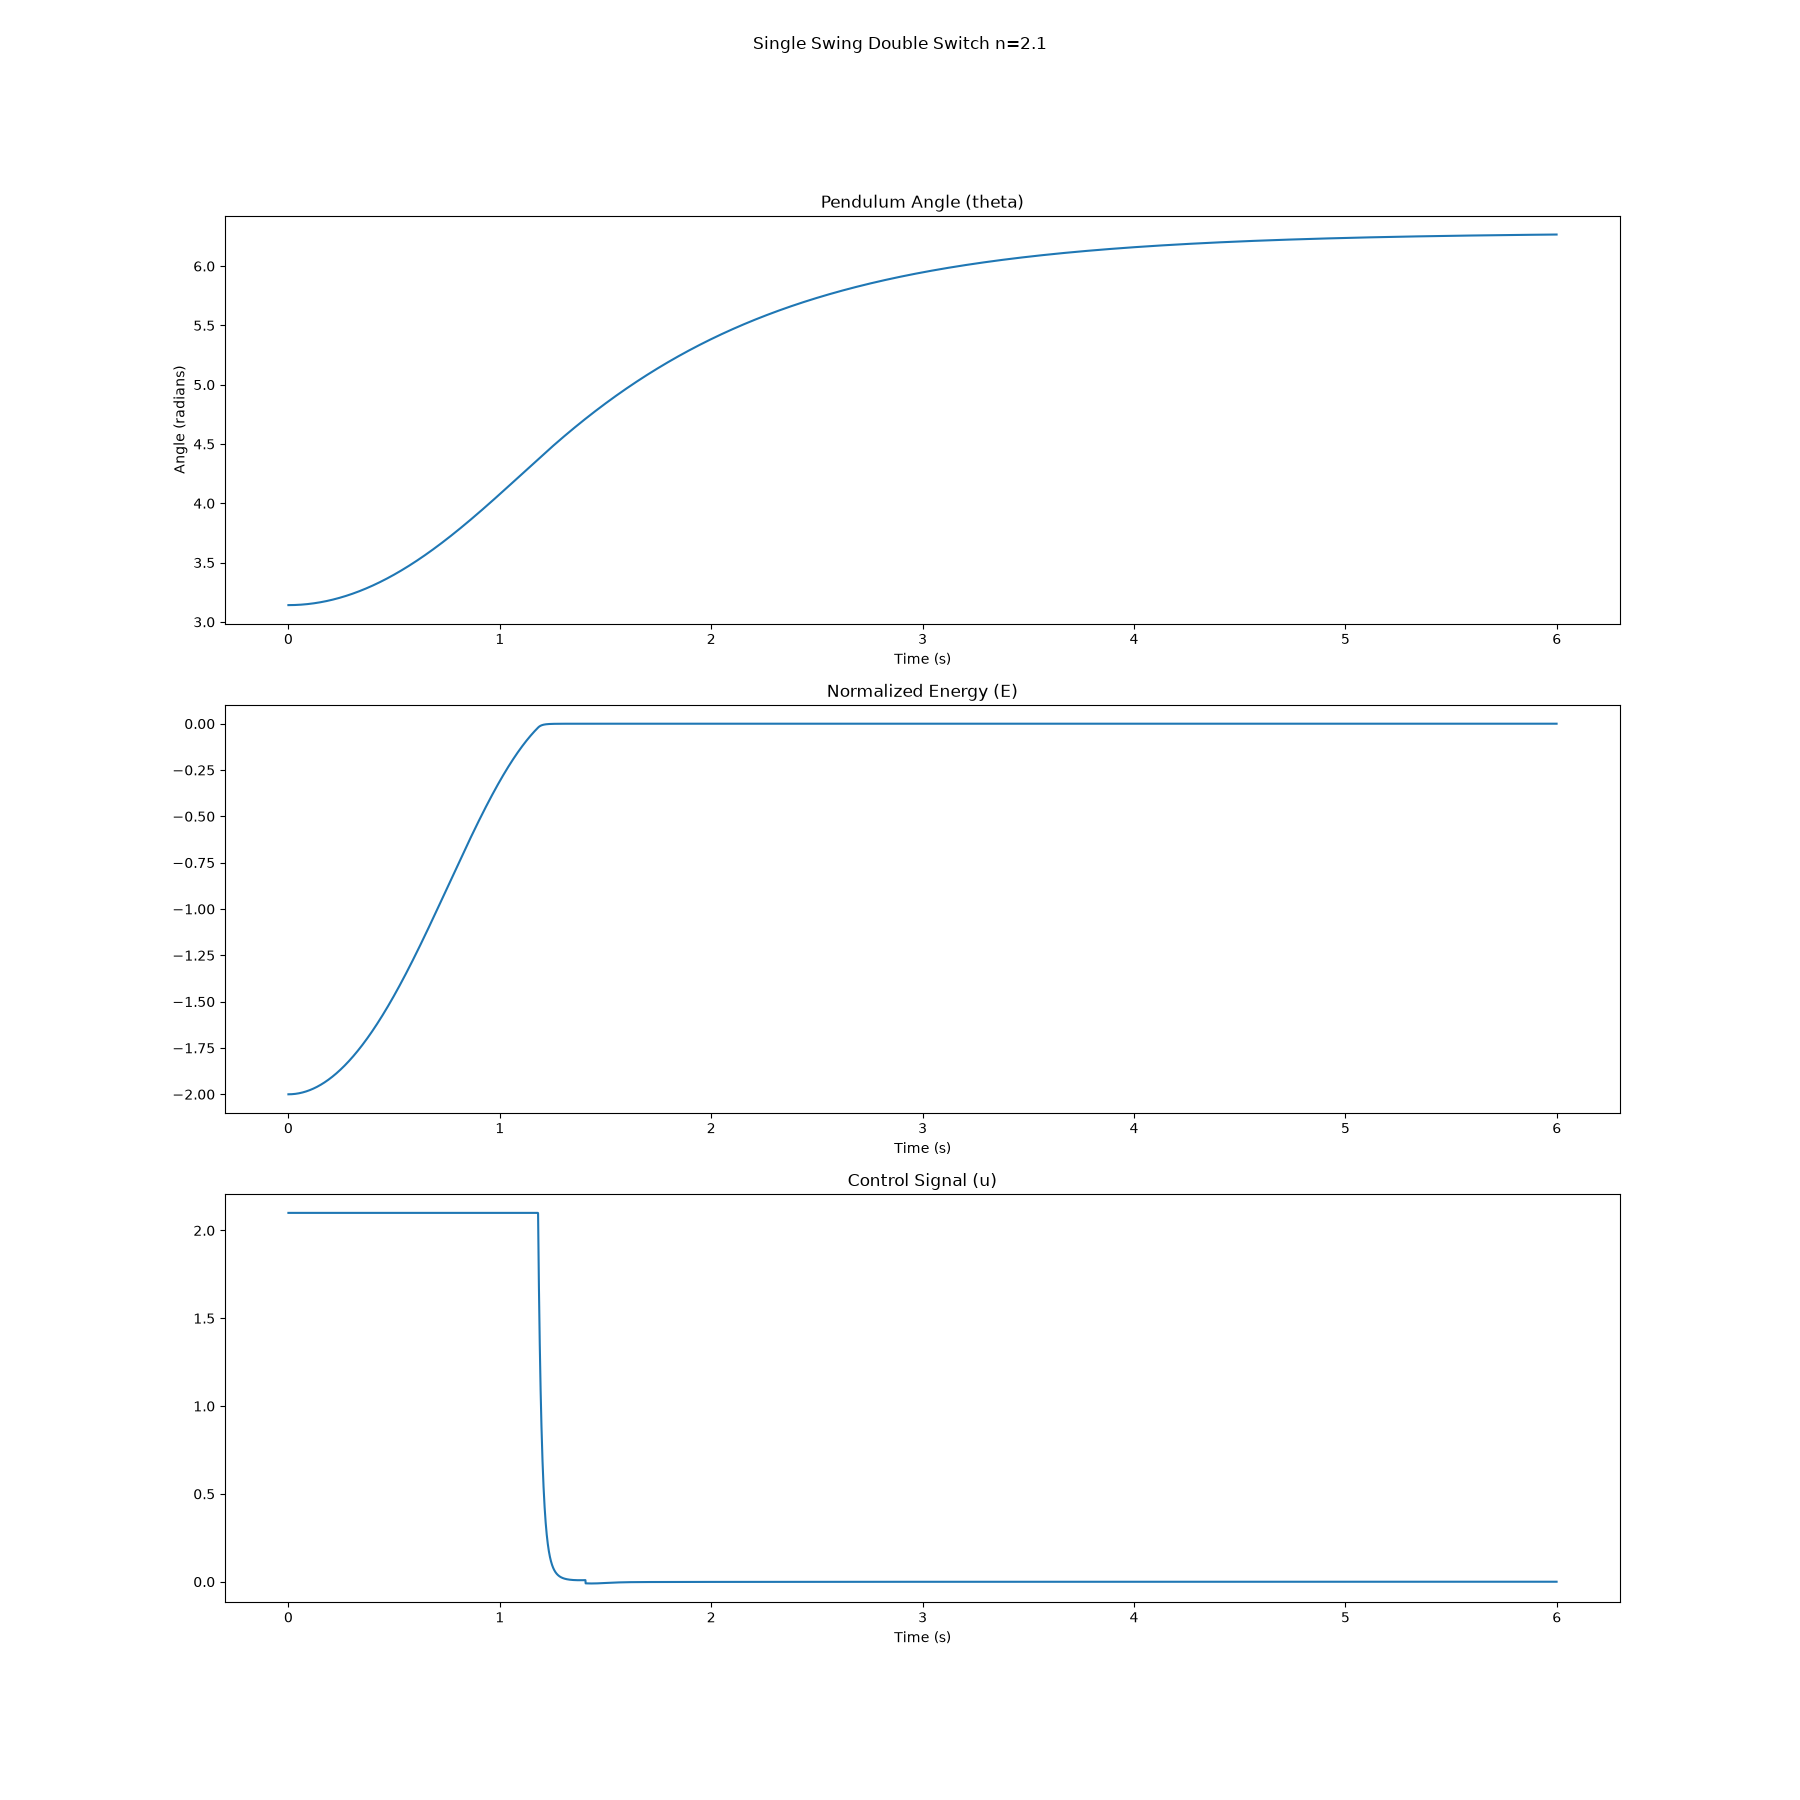
\includegraphics[width=\textwidth]{project1/Single_Swing_Double_Switch_n_2.1_plots.png}
    \caption{Single Swing, Double Switch}
    \label{fig:ssds}
\end{figure}

\subsubsection{Single Swing, Triple Switch}

If $n\leq 2$, we have enough energy to get to the horizontal position, but we need to add more energy to continue the pendulum motion upward. This means we can add one more switch (thus, the name triple switch). The control flow is shown in Table \ref{tab:ssts}.
\begin{table}[ht]
  \centering
  \caption{Single-Swing, Triple-Switch}
  \label{tab:ssts}
  \begin{tabular}{|l|c|c|c|}
    \hline
    Phase & $\theta$ & $u$ & $E_n$ \\
    \hline
    Start & $\pi$ & $0$ & $-2$ \\
    Swing Up & $\pi \rightarrow \frac{\pi}{2}$ & $ng$ & $-2 \rightarrow -2 + n$ \\
    Push Up & $\frac{\pi}{2} \rightarrow \theta^*$ & $-ng$ & $-2 + n \rightarrow 0$ \\
    Coast to Upright & $\theta^* \rightarrow 0$ & $0$ & $0$ \\
    \hline
  \end{tabular}
\end{table}

However, to figure out the bottom threshold of $n$ for this strategy, we can calculate the energy and work done at each phase. Variable $a$ is defined as the distance between the start and $a=\sin{\theta_0} - \cos{\theta_0}$ and $b=1-\sin{\theta_0}$

\begin{align}
    a & \geq b \label{eq:ten} \\
    \sin{\theta_0} - \cos{\theta_0} & \geq 1 - \sin{\theta_0} \notag \\ 
    2\sin{\theta_0} & \geq 1 + \cos{\theta_0} \label{eq:eleven} \\
    2 \frac{n}{\sqrt{1+n^2}} & \geq 1 + \frac{1}{\sqrt{1 + n^2}} \notag \\
    2n &= \sqrt{1 +n^2} +1 \notag \\
    2n-1 &= \sqrt{1+n^2} \notag \\
    4n^2-4n+1 &= 1+n^2 \notag \\
    n(3n-4) &= 0 \notag \\
    \Aboxed{n = \frac{4}{3}} \notag
\end{align}

This means the pivot acceleration must at least be $\frac{4g}{3}$ in order to do the Single Swing, Triple Switch strategy.

Using equation \eqref{eq:eleven}, we can find $\theta_0$:
\begin{align*}
    n &= \tan{\theta_0} \\
    \Aboxed{\theta_0 &= \arctan{n}}
\end{align*}
To calculate the angle when the pivot acceleration should be set to zero, $\theta^*$, we can use the fact that the sum of work must also equal $2mgl$, the upright position.

\begin{align*}
    W_1 + W_2 &= 2mgl \\
    mngl + mngl(1-\sin{\theta^*}) &= \\
    mngl(2 - \sin{\theta^*}) &= 2mgl \\
    n(2 - \sin{\theta^*}) &= 2 \\
    \sin{\theta^*} &= 2-\frac{2}{n} \\
    \Aboxed{\theta^* &= \arcsin{\left(2-\frac{2}{n}\right)}}
\end{align*}

We reproduce the simulation for SSTS with $w_0=1$, using equation \eqref{eq:eight} for control law, $n=1.5$, and $k=100$. Results are shown in Figure \ref{fig:ssts}.

\begin{figure}[htbp]
    \centering
    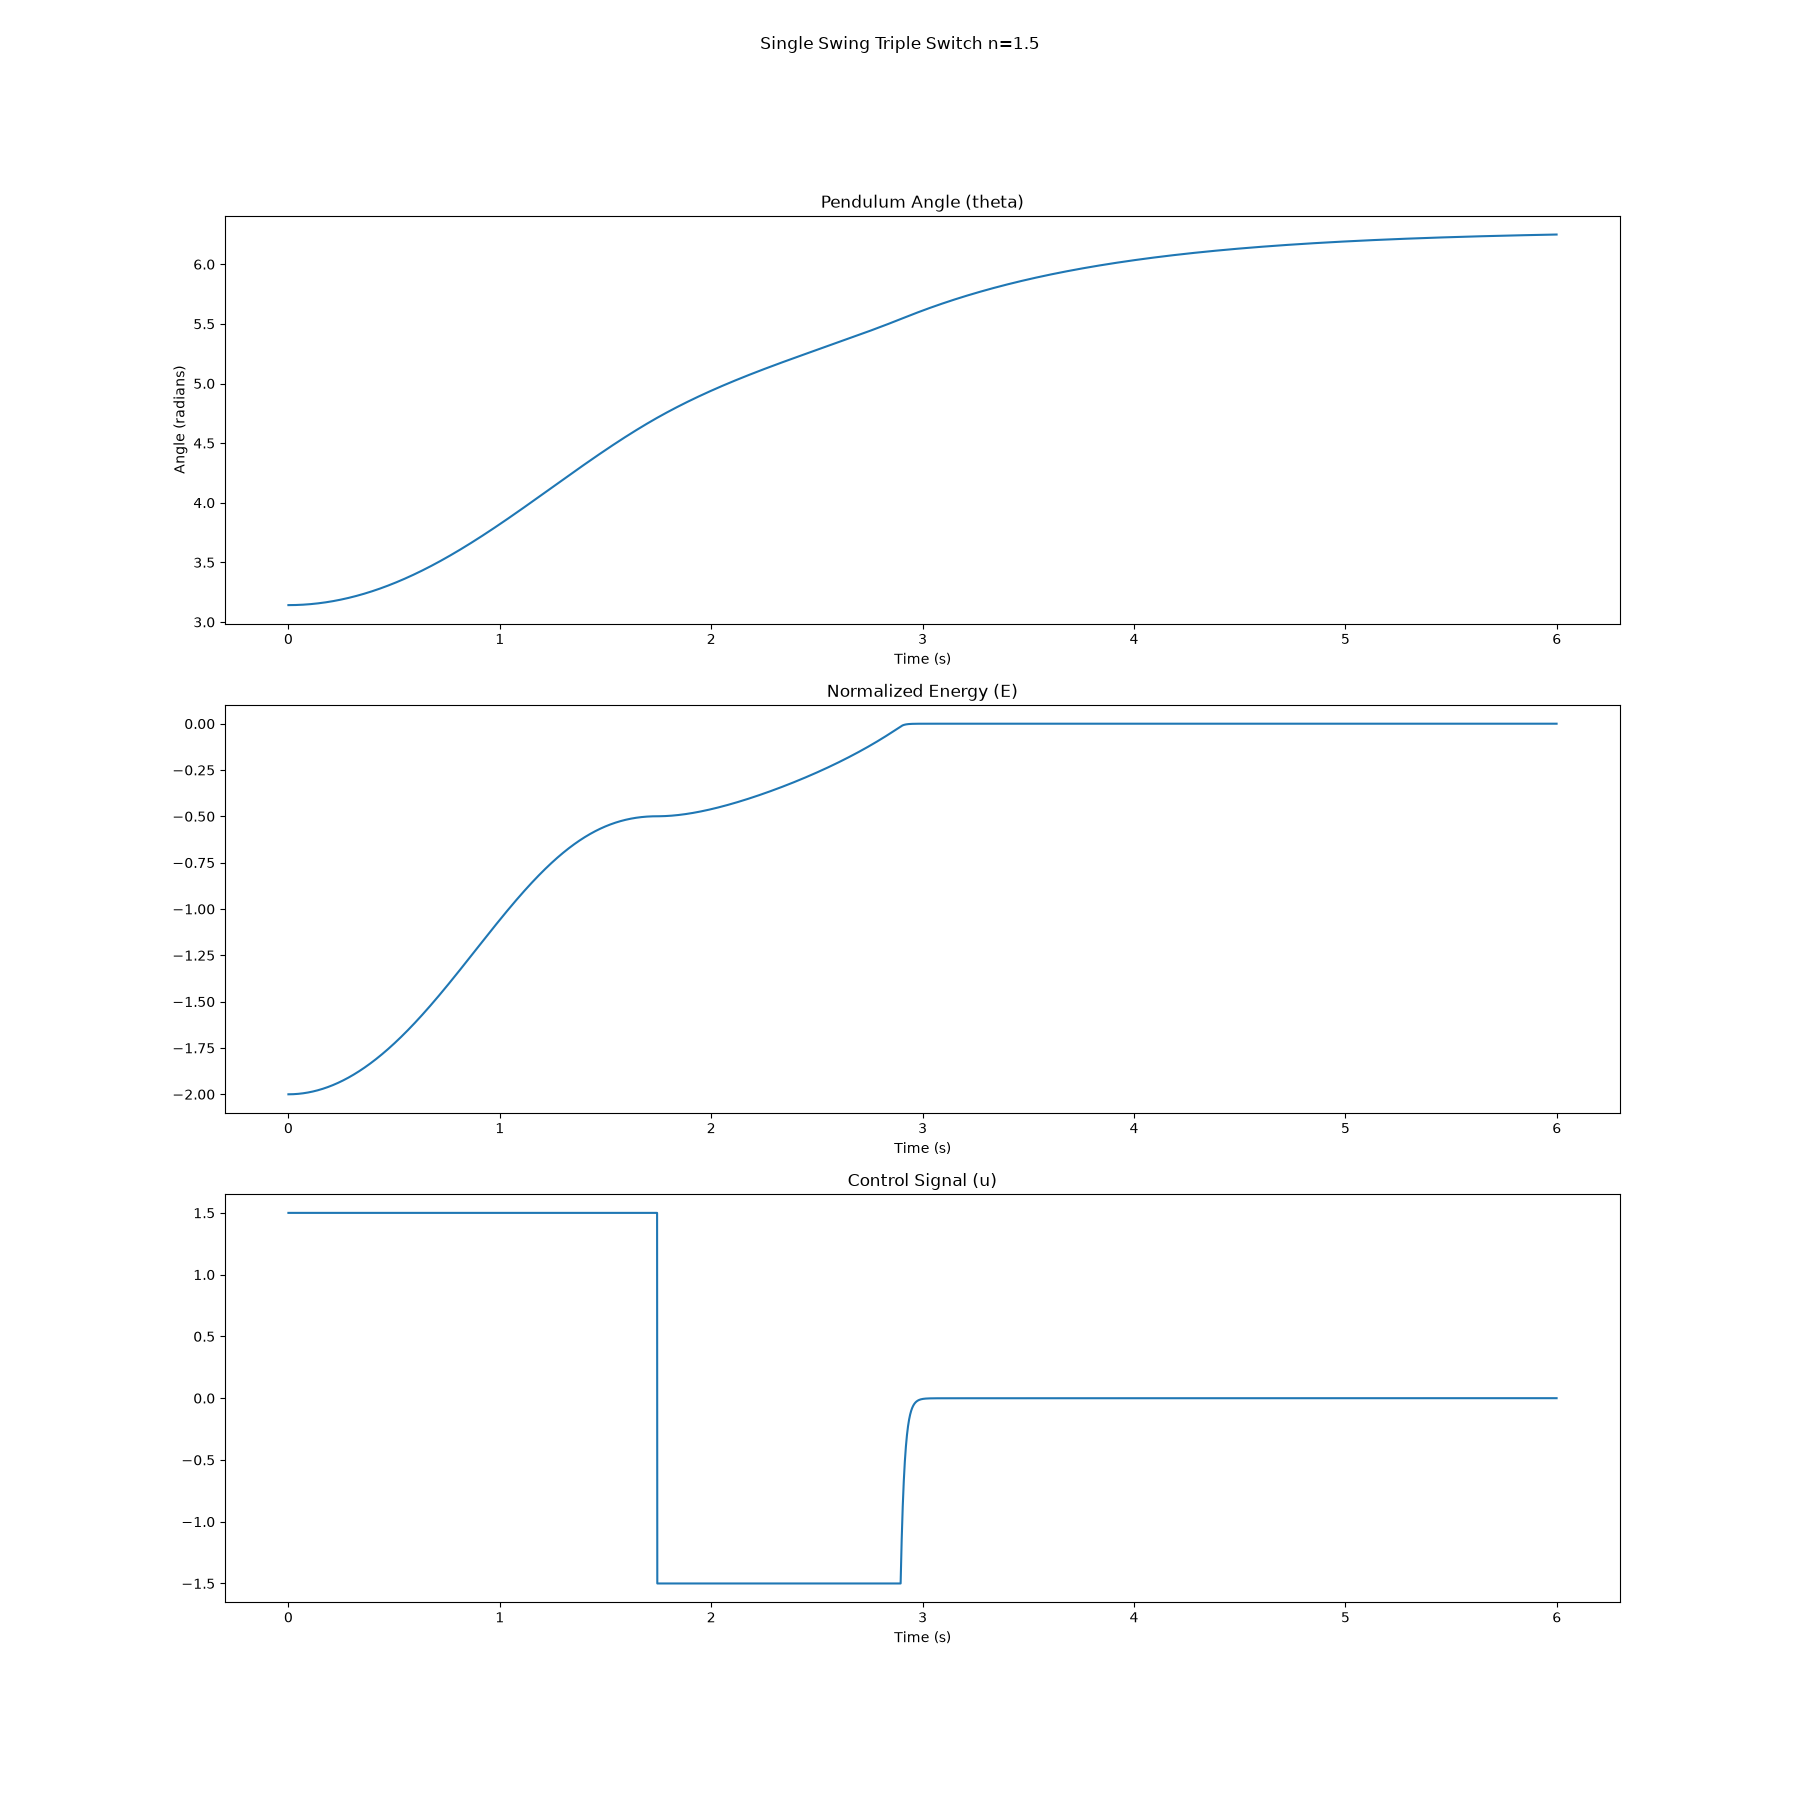
\includegraphics[width=\textwidth]{project1/Single_Swing_Triple_Switch_n_1.5_plots.png}
    \caption{Single Swing, Triple Switch}
    \label{fig:ssts}
\end{figure}

\subsubsection{Multiple Swings}
In the case where $n < \frac{4}{3}$, we need multiple swings of the pendulum to bring the pendulum up.

Each time the pendulum comes to rest, $\dot{\theta}\cos\theta$ changes sign, so the control law reverses the pivot acceleration. The effective gravity field then tilts by $\theta_0$ to the opposite side, and because the pendulum swings symmetrically about the field direction, each swing ends $2\theta_0$ further from the bottom than the previous one. 

\begin{align}
    2\sin{\theta_0} & \geq 1 + \cos{3}\theta_0 && \text{For two swings} \label{eq:twelve} \\
    2\sin{\theta_0} & \geq 1 + \cos{\left((2j - 1)\theta_0\right)} && \text{For j swings} \label{eq:thirteen}
\end{align}

After $j$ swings the pendulum is at rest at $|\varphi_j| = 2j\theta_0$, with normalized energy
\begin{align*}
    E_n = \cos\theta - 1 = -1 - \cos(2j\theta_0).
\end{align*}

A summary of this strategy is shown in Table \ref{tab:multiswing}.

\begin{table}[ht]
  \centering
  \caption{Multiple Swings ($k$ swings, $n < \frac{4}{3}$)}
  \label{tab:multiswing}
  \begin{tabular}{|l|c|c|c|}
    \hline
    Phase & $\varphi$ & $u$ & $E_n$ \\
    \hline
    Start & $0$ & $0$ & $-2$ \\
    Swing 1 & $0 \rightarrow 2\theta_0$ & $ng$ & $-2 \rightarrow -1-\cos 2\theta_0$ \\
    Swing 2 & $2\theta_0 \rightarrow -4\theta_0$ & $-ng$ & $\rightarrow -1-\cos 4\theta_0$ \\
    $\vdots$ & $\vdots$ & $\vdots$ & $\vdots$ \\
    Swing $j$ & $\rightarrow (-1)^{j+1}\, 2j\theta_0$ & $(-1)^{j+1}\, ng$ & $\rightarrow -1-\cos 2j\theta_0$ \\
    $\vdots$ & $\vdots$ & $\vdots$ & $\vdots$ \\
    Final swing $k$, to horizontal & $\rightarrow \pm\frac{\pi}{2}$ & $(-1)^{k+1}\, ng$ & increasing \\
    Final swing $k$, past horizontal & $\pm\frac{\pi}{2} \rightarrow \varphi^*$ & $(-1)^{k}\, ng$ & $\rightarrow 0$ \\
    Coast to Upright & $\varphi^* \rightarrow \pm\pi$ & $0$ & $0$ \\
    \hline
    \multicolumn{4}{|l|}{Final swing succeeds if $2\sin\theta_0 \geq 1 + \cos\big((2k-1)\theta_0\big)$, Eq.~(13)} \\
    \hline
  \end{tabular}
\end{table}

We recreate the results for five swings, with $n=0.25$, $w_0=1$, $k=100$, and control equation \eqref{eq:eight}, as seen in Figure \ref{fig:ms}.

\begin{figure}[htbp]
    \centering
    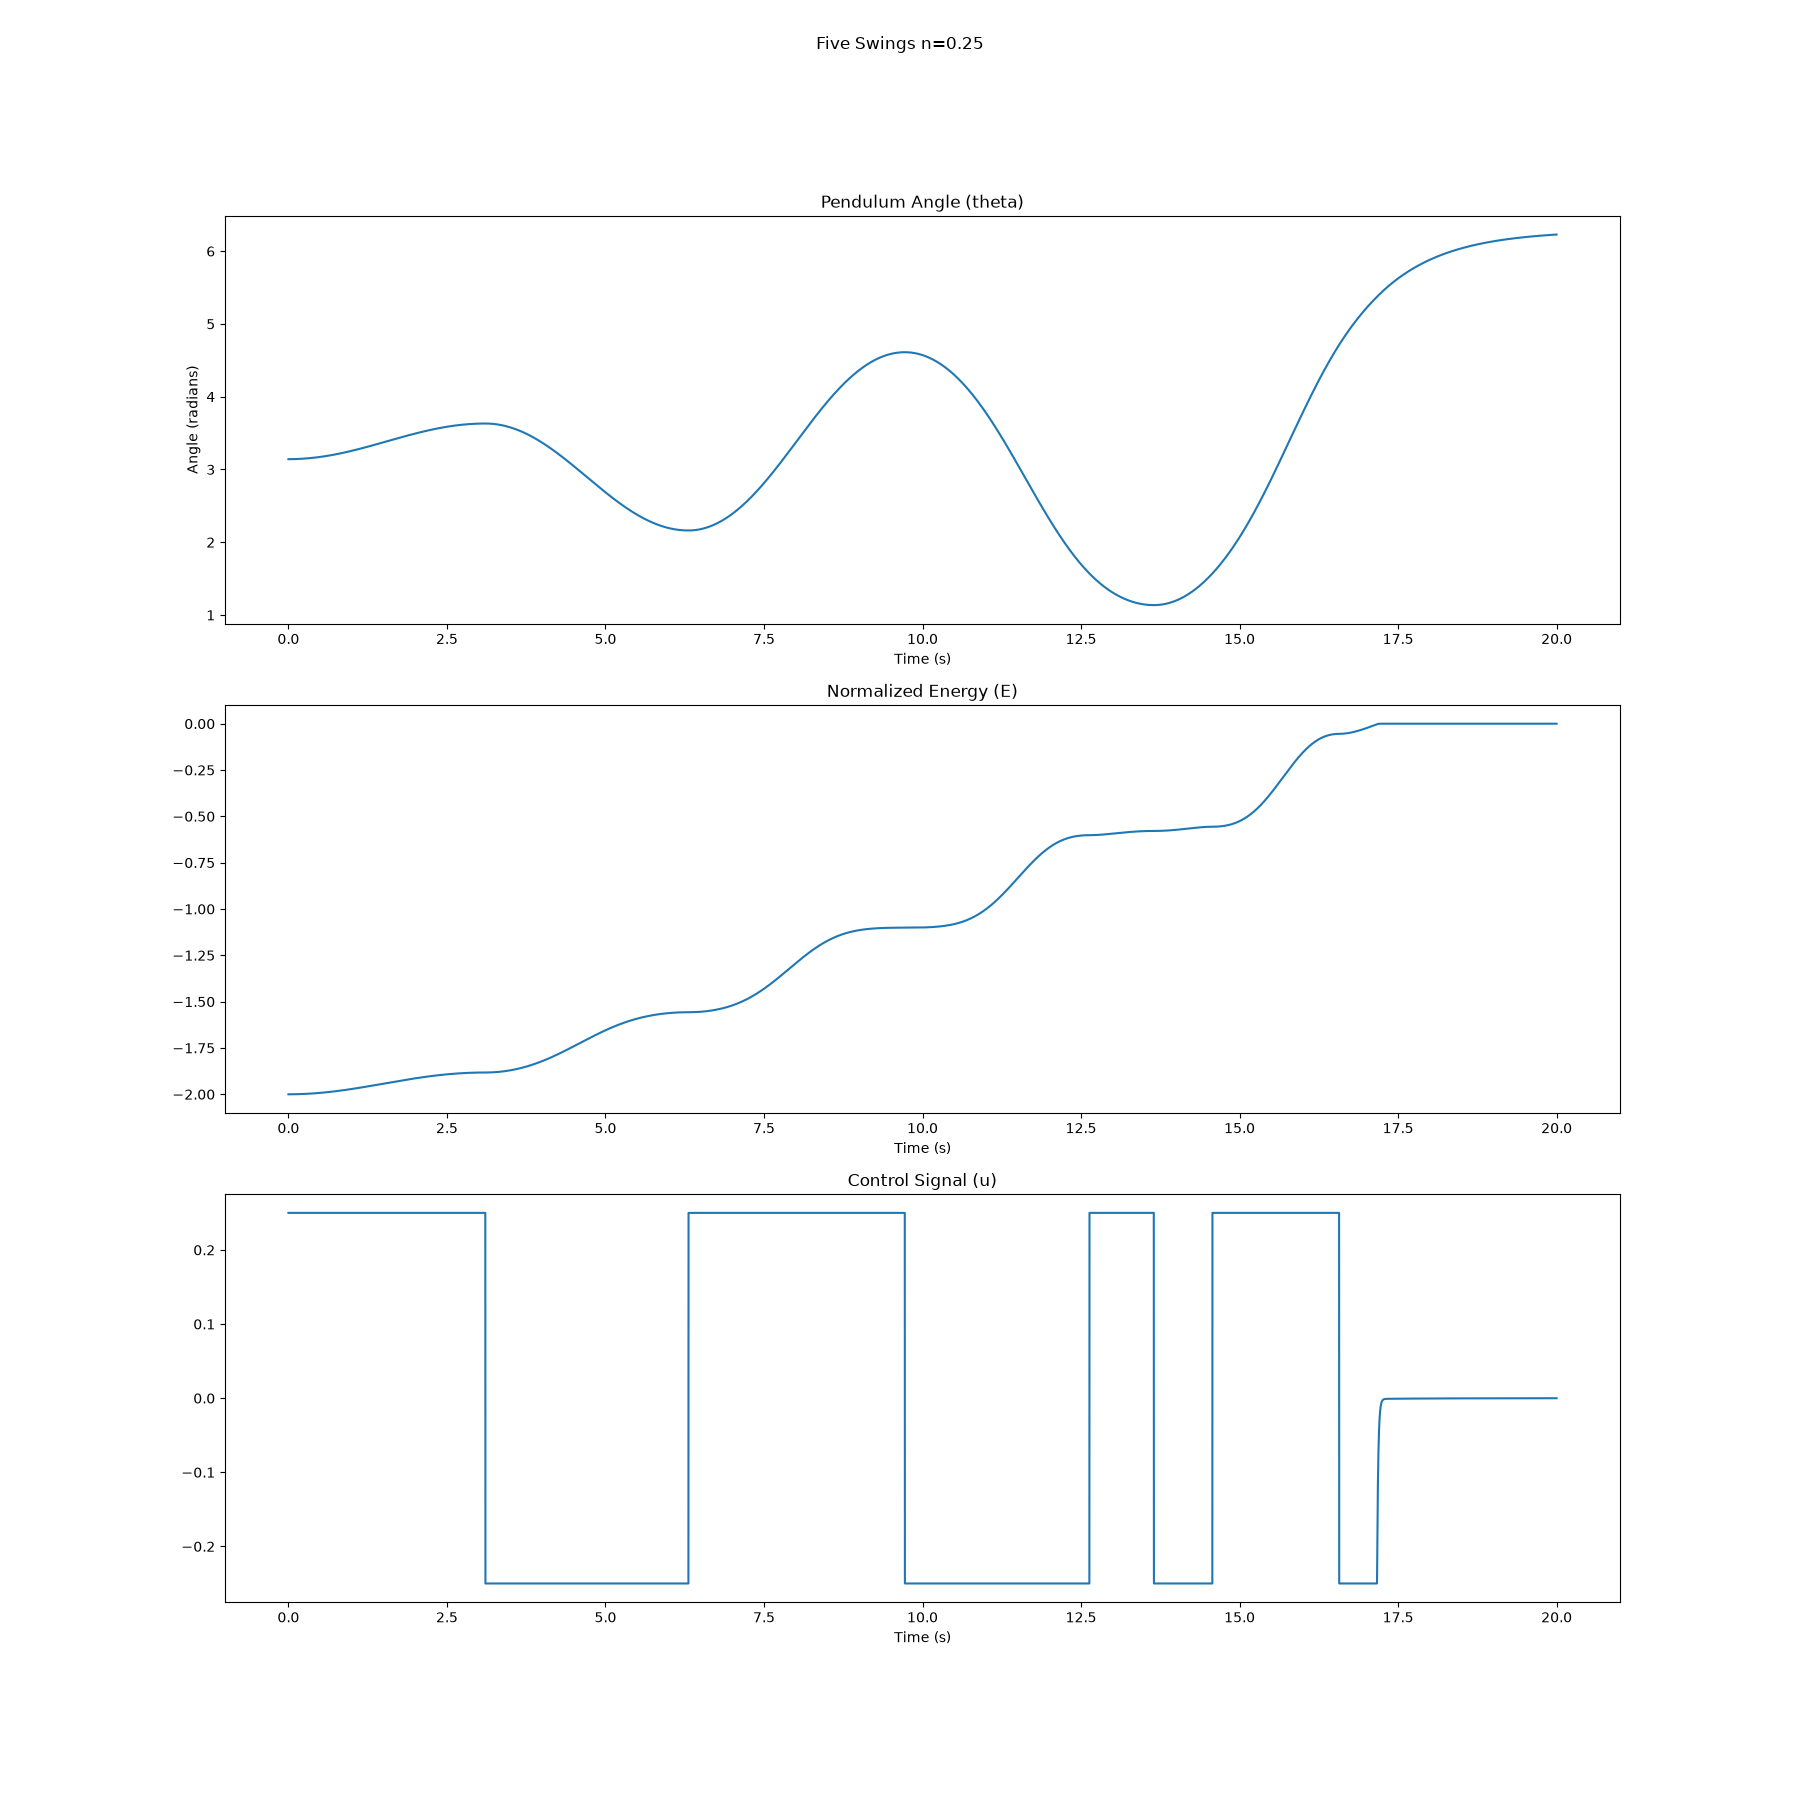
\includegraphics[width=\textwidth]{project1/Five_Swings_n_0.25_plots.png}
    \caption{5 Swings}
    \label{fig:ms}
\end{figure}

\subsubsection{Minimum Time}
According to Pontryagin's maximum principle, the fastest way to get the pendulum upright is to use bang-bang type control (rapidly switching between maximum values). What this looks like is moving the pivot at maximal acceleration ($ng$) to quickly get the pendulum, then brake the pendulum motion to not overshoot the upright position, as seen in Table \ref{tab:mt}.

\begin{table}[ht]
  \centering
  \caption{Minimum Time ($n \geq 2$)}
  \label{tab:mt}
  \begin{tabular}{|l|c|c|c|}
    \hline
    Phase & $\theta$ & $u$ & $E_n$ \\
    \hline
    Start & $-\pi$ & $0$ & $-2$ \\
    Swing Up & $-\pi \rightarrow -\frac{\pi}{2}$ & $ng$ & $-2 \rightarrow -2 + n$ \\
    Push Up & $-\frac{\pi}{2} \rightarrow -\theta^*$ & $-ng$ & $-2 + n \rightarrow n - 1$ \\
    Brake to Upright & $-\theta^* \rightarrow 0$ & $ng$ & $n - 1 \rightarrow 0$ \\
    Upright & $0$ & $0$ & $0$ \\
    \hline
    \multicolumn{4}{|l|}{$\theta^* = \arcsin\!\left(1 - \frac{1}{n}\right)$, measured from vertical; peak energy $E_{max} = (n-1)\,mgl$} \\
    \hline
  \end{tabular}
\end{table}

By summing up the work at each phase, we can determine what angle thresholds are needed for the control. More specifically, $\theta^*$, when to apply the brakes by changing $u$ from $-ng$ to $ng$.

\begin{align*}
    W_1 + W_2 - W_3 &= 2mgl \\
    mngl + mngl(1-\sin{\theta^*}) - mngl\sin{\theta^*} &= 2mgl \\
    n + n(1-\sin{\theta^*}) - n\sin{\theta^*} &= 2 \\
    -2n\sin{\theta^*} &= 2-2n
    \sin{\theta^*} &= 1 - \frac{1}{n} \\
    \Aboxed{\theta^* &= \arcsin{\left(1-\frac{1}{n}\right)}}
\end{align*}

This gives us a maximum energy of:
\begin{align}
    E_{max} &= nmgl\sin{\theta^*} \notag \\
    E_{max} &= mgl(n-1) \label{eq:fourteen}
\end{align}

We simulate $n=2.1$ and $n=5$ for minimum time, and also compare it with our previous Single Swing Double Switch strategies, seen in Figures \ref{fig:mt1} and \ref{fig:mt2}.

\begin{figure}[htbp]
    \centering
    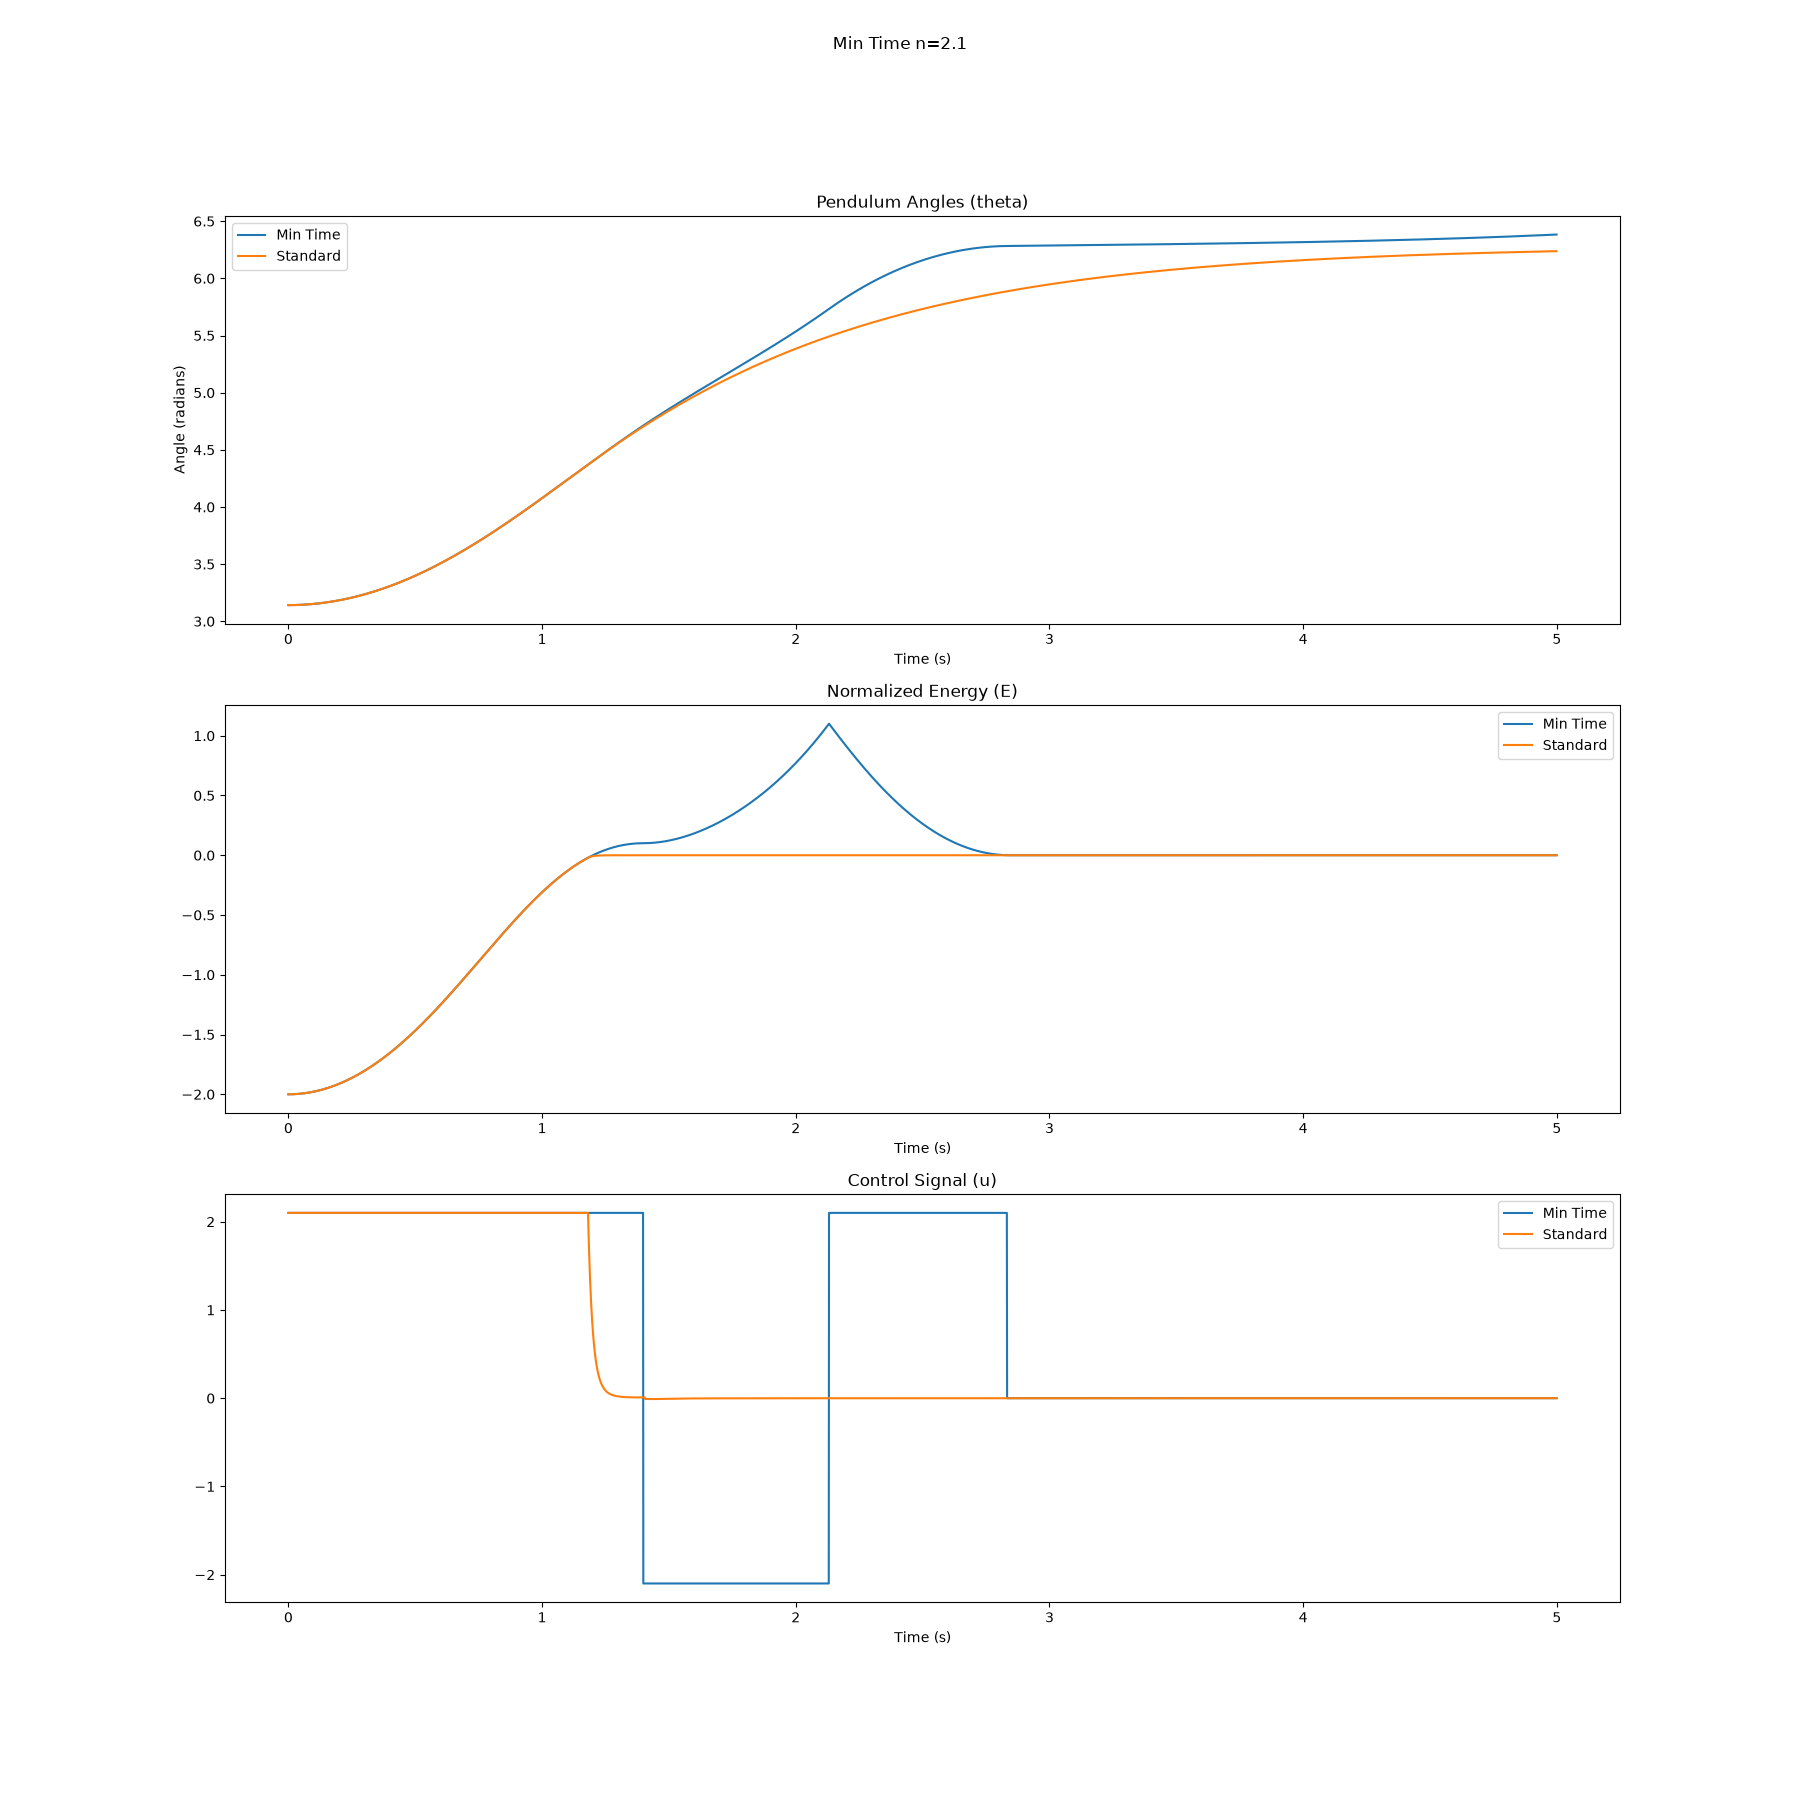
\includegraphics[width=\textwidth]{project1/Min_Time_n_2.1_plots.png}
    \caption{Minimum Time n=2.1}
    \label{fig:mt1}
\end{figure}

\begin{figure}[htbp]
    \centering
    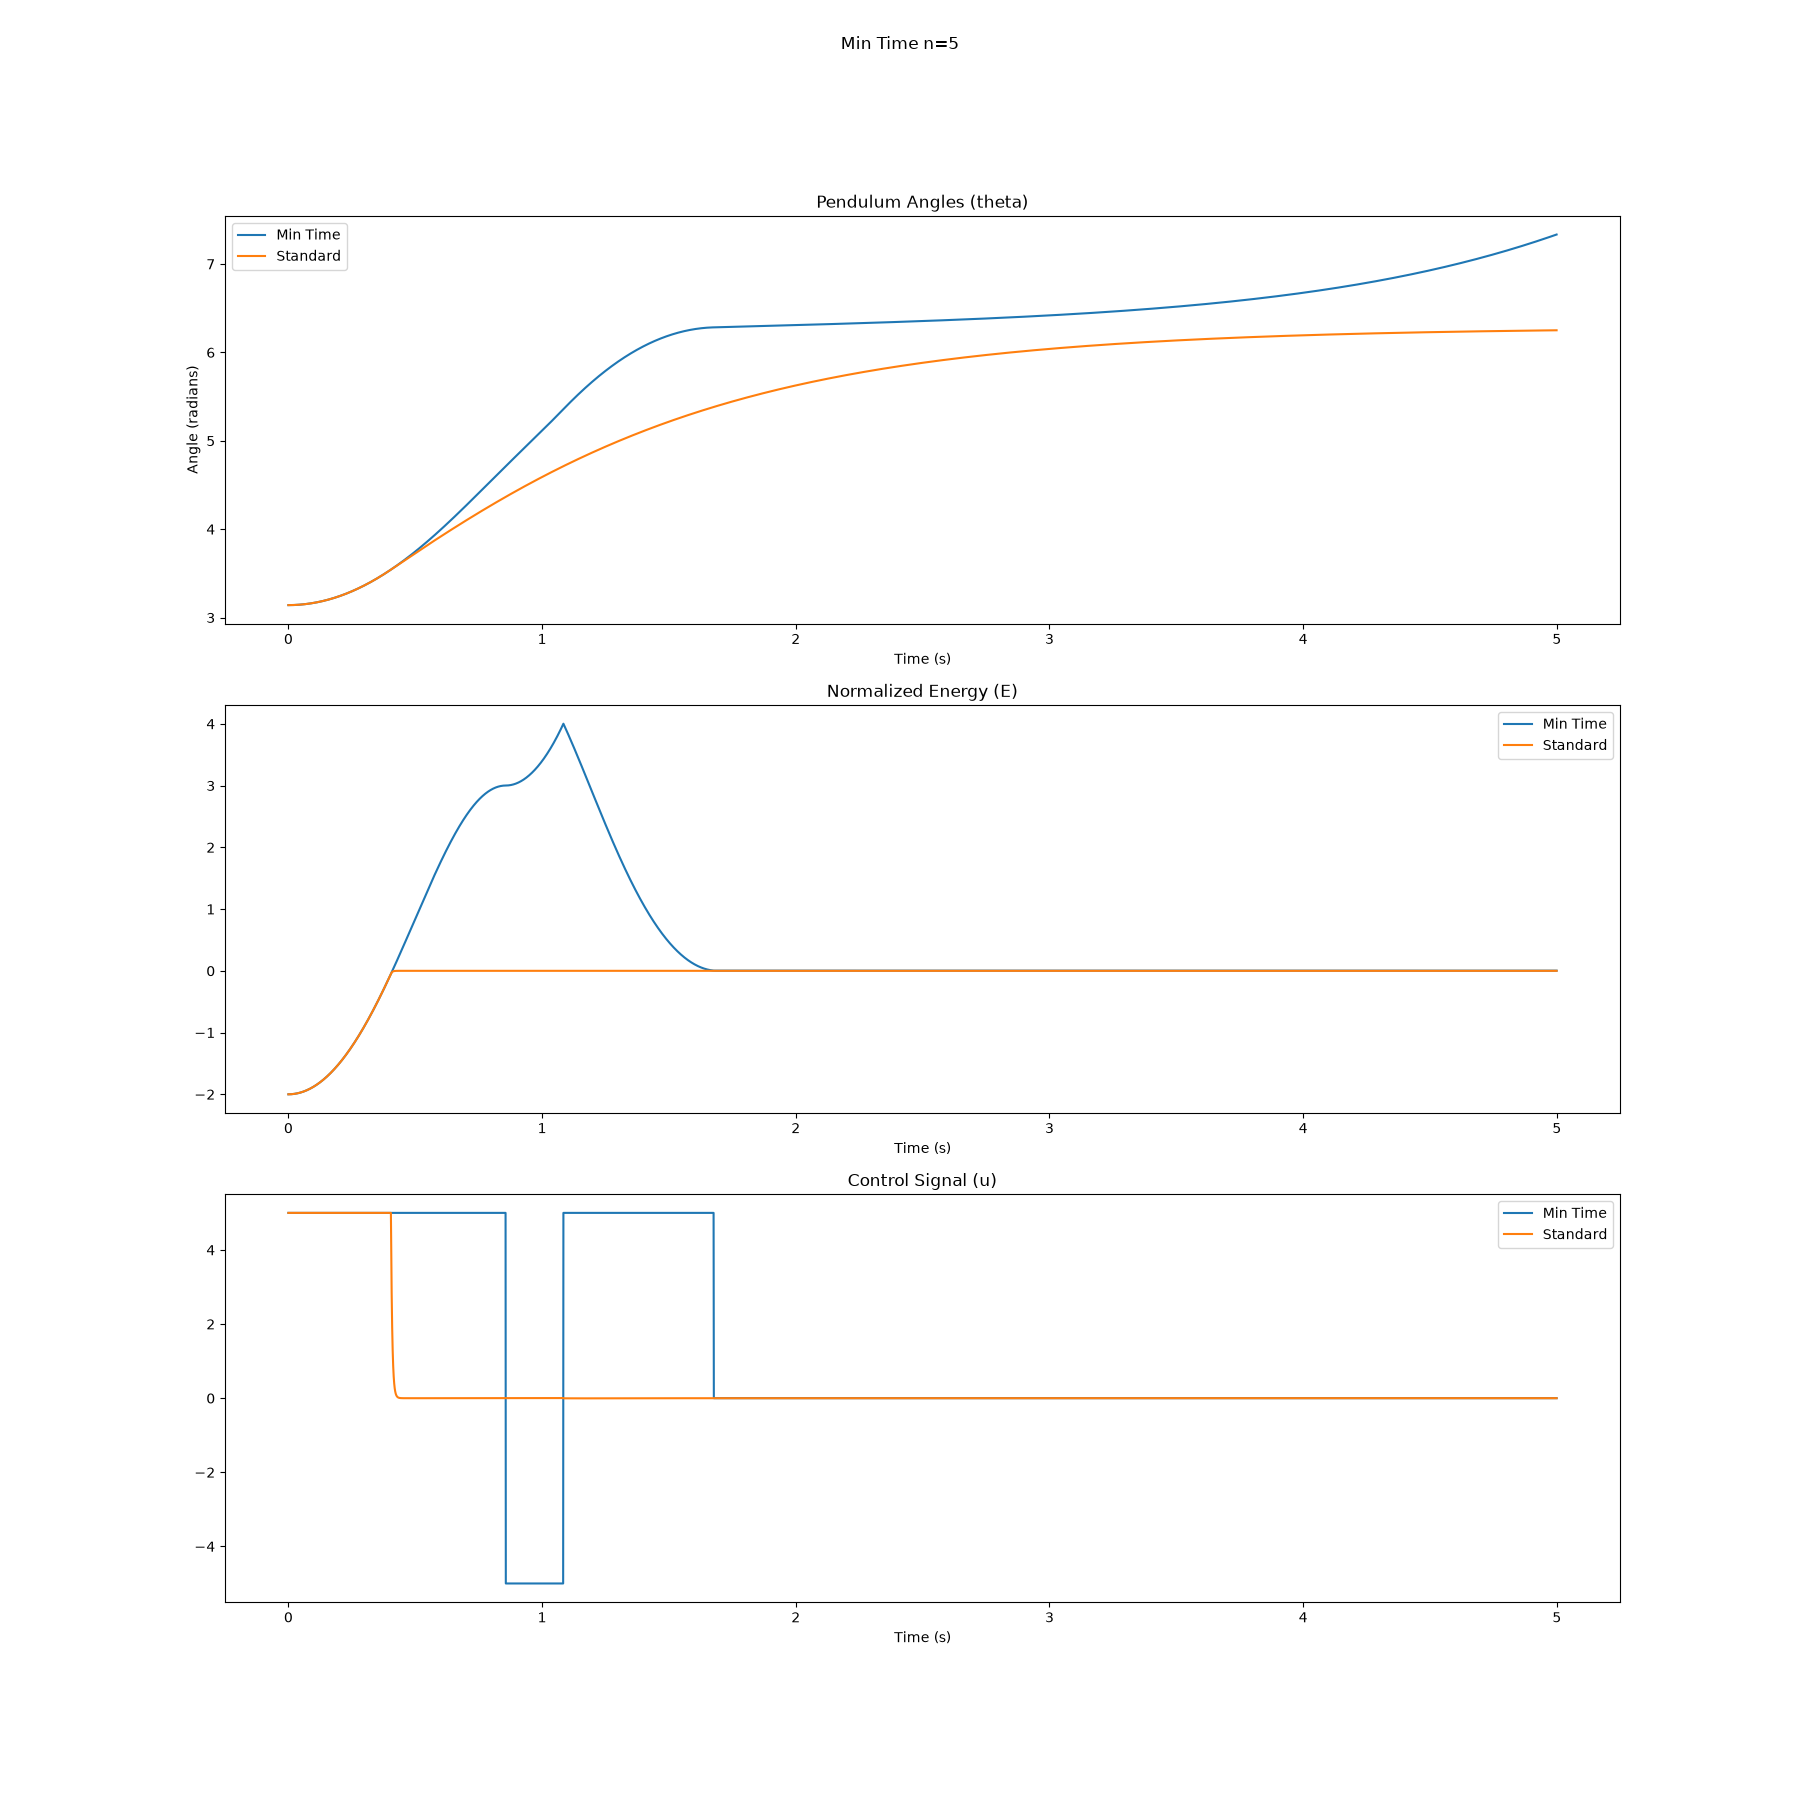
\includegraphics[width=\textwidth]{project1/Min_Time_n_5_plots.png}
    \caption{Minimum Time n=5}
    \label{fig:mt2}
\end{figure}

\subsubsection{Two Pendulums}
The authors extend their control and analysis to multiple pendulums coupled to the same pivot/cart. 

\subsubsection{General Mechanical Systems}
The authors first extend energy control to a general mechanical system with generalized coordinates $q$, inertia matrix $M(q,\dot{q})$, Coriolis/damping matrix $C(q,\dot{q})$, potential energy $U(q)$, and external control torques $T$:
\begin{align}
    M(q,\dot{q})\ddot{q} + C(q,\dot{q})\dot{q} + \frac{\partial U(q)}{\partial q} &= T \label{eq:fifteen}
\end{align}

The total energy is
\begin{align}
    E &= \frac{1}{2}\dot{q}^{T}M(q,\dot{q})\dot{q} + U(q) \label{eq:sixteen}
\end{align}

Differentiating with respect to time and substituting $M\ddot{q}$ from \eqref{eq:fifteen}:
\begin{align}
    \frac{dE}{dt} &= \dot{q}^{T}M\ddot{q} + \frac{1}{2}\dot{q}^{T}\dot{M}\dot{q} + \left(\frac{\partial U}{\partial q}\right)^{T}\dot{q} \notag \\
    &= \dot{q}^{T}\left(T - C\dot{q} - \frac{\partial U}{\partial q}\right) + \frac{1}{2}\dot{q}^{T}\dot{M}\dot{q} + \left(\frac{\partial U}{\partial q}\right)^{T}\dot{q} \notag \\
    &= \frac{1}{2}\dot{q}^{T}\left(\dot{M}(q,\dot{q}) - 2C(q,\dot{q})\right)\dot{q} + T^{T}\dot{q} \label{eq:seventeen}
\end{align}

Since $\dot{M} - 2C$ is skew-symmetric \cite{spong1989robot}, $\dot{q}^{T}(\dot{M} - 2C)\dot{q} = 0$, and therefore
\begin{align*}
    \frac{dE}{dt} = T^{T}\dot{q}.
\end{align*}
The rate of change of energy depends only on the control torques, and we can use the energy control the authors propose.

\subsubsection{Two Pendulums}
For two pendulums mounted on the same cart, both driven by the same pivot acceleration $u$. Applying equation \eqref{eq:five} to each pendulum separately gives
\begin{align}
    \frac{dE_1}{dt} &= -m_1 u l_1 \dot{\theta}_1 \cos\theta_1 \notag \\
    \frac{dE_2}{dt} &= -m_2 u l_2 \dot{\theta}_2 \cos\theta_2 \label{eq:eighteen}
\end{align}

We apply similar analysis using Lyapunov function to determine what is a good control law:
\begin{align*}
    V &= \frac{1}{2}\left(E_1^2 + E_2^2\right) \\
    \frac{dV}{dt} &= E_1\frac{dE_1}{dt} + E_2\frac{dE_2}{dt} \\
    &= -u\left(m_1 l_1 E_1 \dot{\theta}_1 \cos\theta_1 + m_2 l_2 E_2 \dot{\theta}_2 \cos\theta_2\right) \\
    &= -Gu,
\end{align*}
We define $G = m_1 l_1 E_1 \dot{\theta}_1 \cos\theta_1 + m_2 l_2 E_2 \dot{\theta}_2 \cos\theta_2$. Choosing formula for u:
\begin{align}
    u &= \operatorname{sat}_{ng}(kG) \label{eq:nineteen}
\end{align}

We simulate $n=1.5$ for two pendulums where $w_01=1$ and $w_02=2$, $k=20$, and using equation \eqref{eq:nineteen} for control law, as shown in Figure \ref{fig:twopen}.

\begin{figure}[htbp]
    \centering
    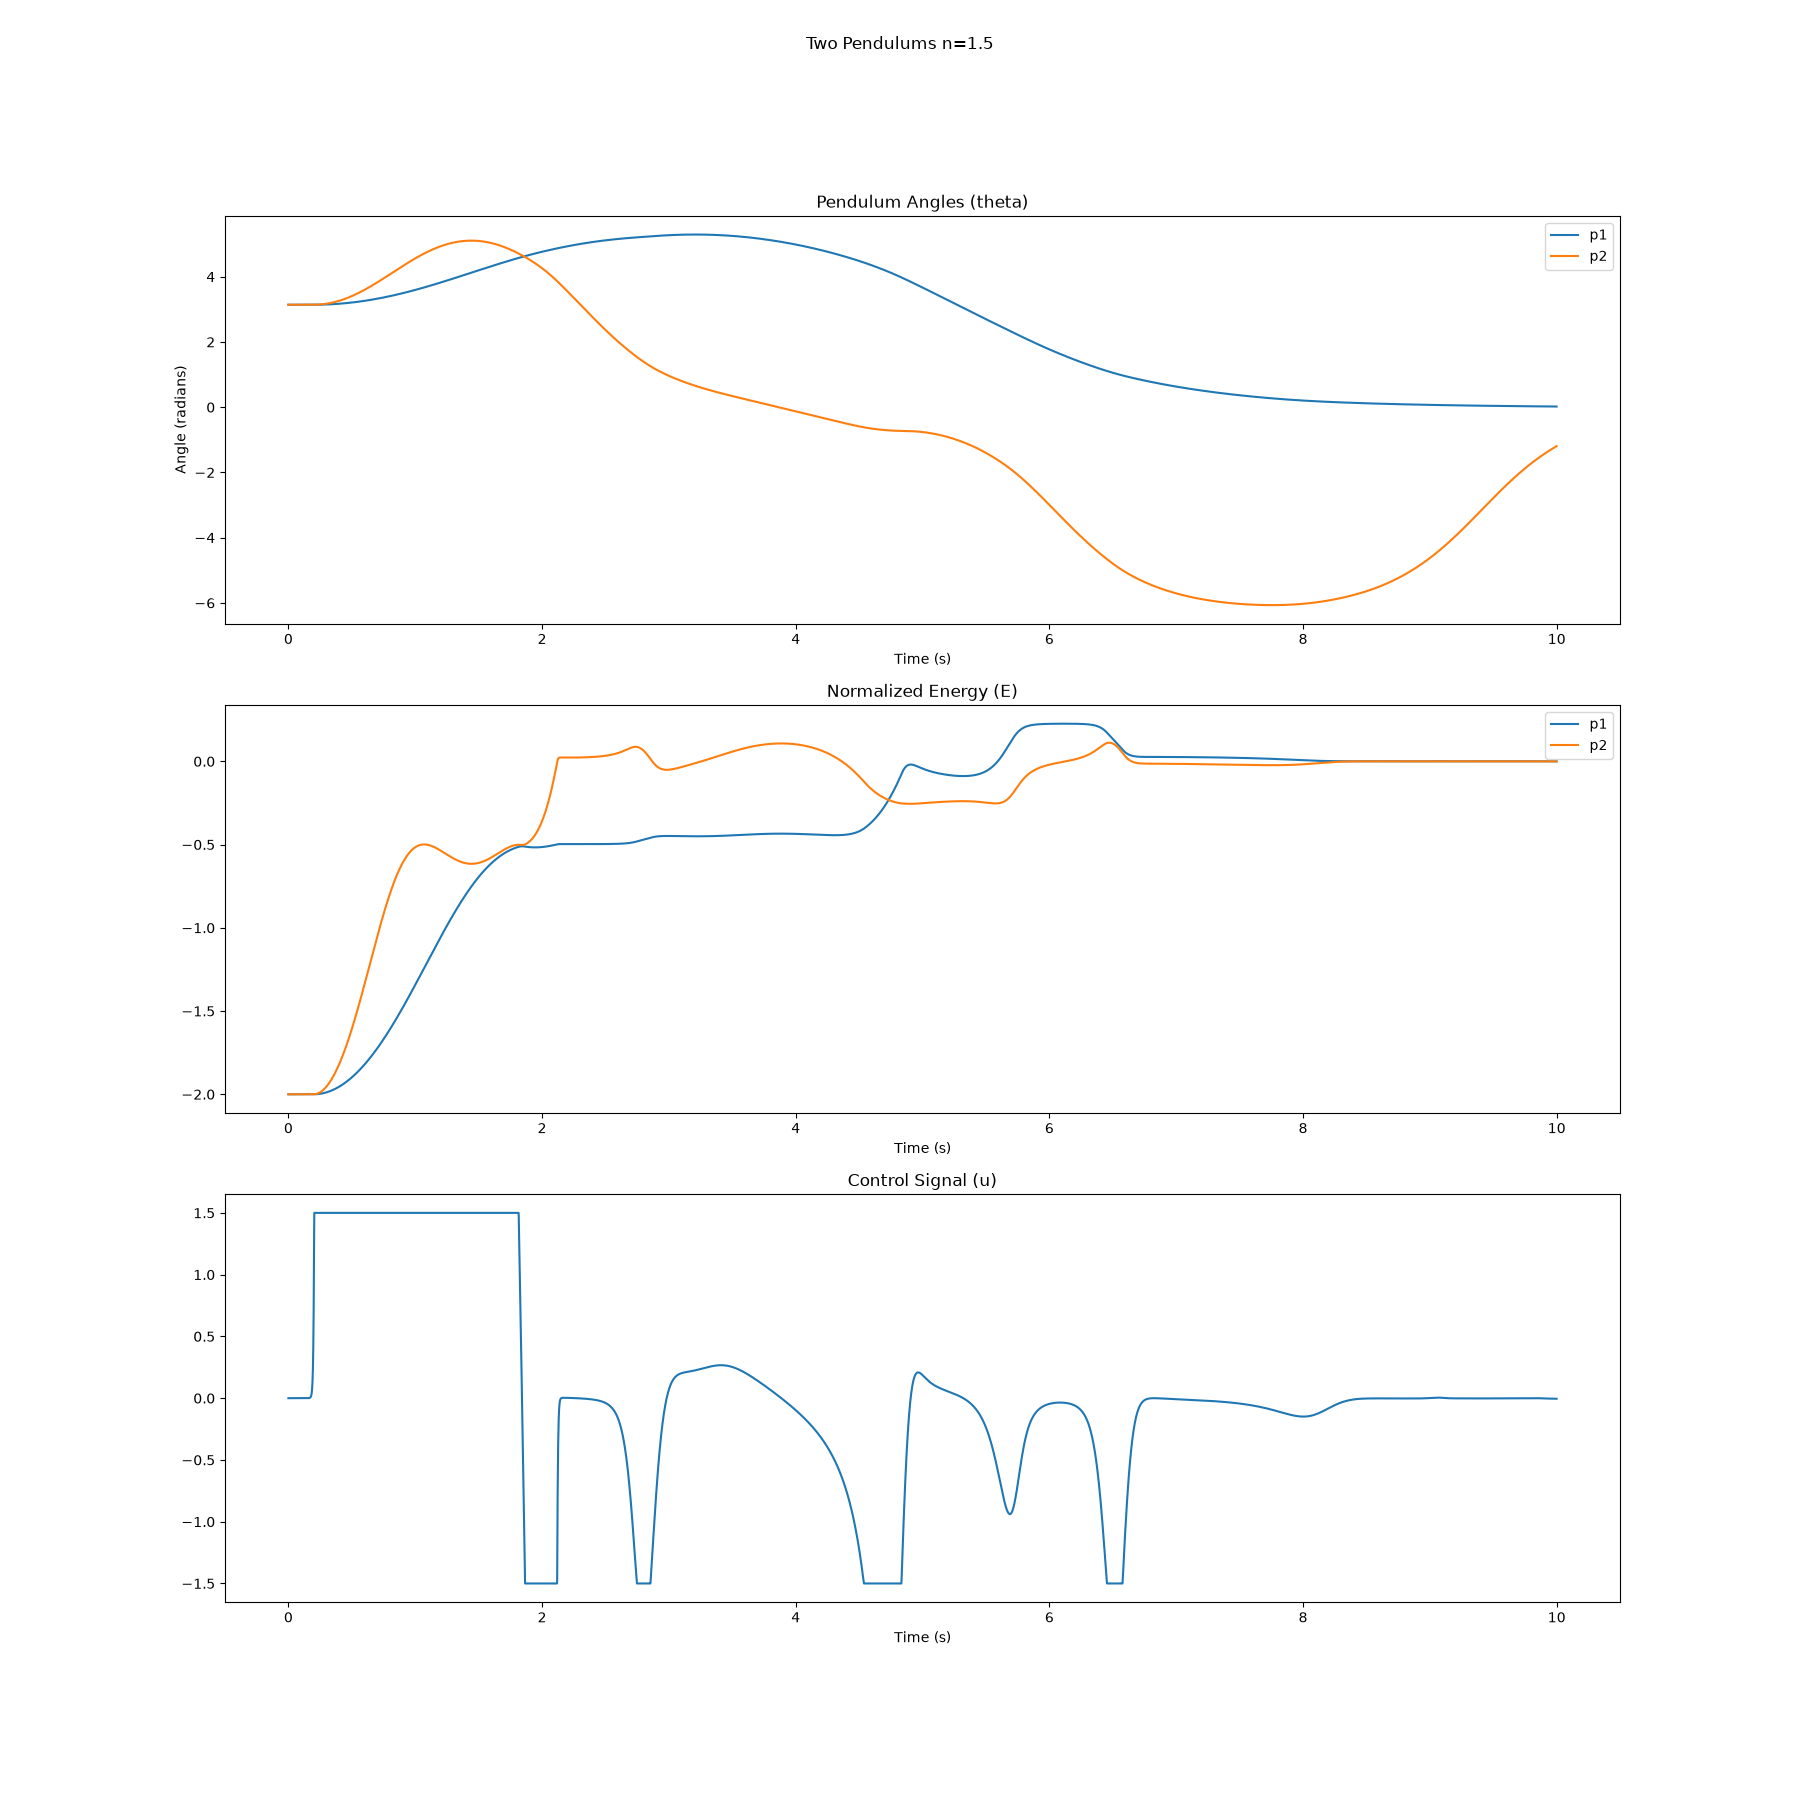
\includegraphics[width=\textwidth]{project1/Two_Pendulums_n_1.5_plots.png}
    \caption{Two Pendulums n=1.5}
    \label{fig:twopen}
\end{figure}

\section{Discussion}
Inverted pendulum swing up strategies depend on what the maximum pivot acceleration is. Table \ref{tab:summary} summarizes $n$ values and what swing-up strategy is used.

\begin{table}[ht]
  \centering
  \caption{Summary of Swing-Up Strategies by Maximum Pivot Acceleration $n$}
  \label{tab:summary}
  \begin{tabular}{|l|c|}
    \hline
    Strategy & $n$ \\
    \hline
    Single Swing, Double Switch & $n \geq 2$ \\
    Single Swing, Triple Switch & $\frac{4}{3} \leq n < 2$ \\
    Multiple Swings ($k$ swings) & $n < \frac{4}{3}$, $k$ from Eq.~(13) \\
    Minimum Time & $n \geq 2$ \\
    \hline
  \end{tabular}
\end{table}

Although we are unable to accurately determine exact differences in the paper results and our results, there will definitely be small differences due to using Euler's method to update pendulum angular acceleration, angular velocity, and $\theta$ numerically.

However, implementing this energy-based control in reality would look a lot different, since friction is ignored, and there is no maximum for pivot velocity.


\section{Conclusion}
Åström \& Furuta effectively prove energy control is possible for the inverted pendulum problem, and it depends on the pivot max acceleration, $u$. If it is large enough, a single swing would be enough. If too small ($n< \frac{4}{3}$), then multiple swings are required. They also demonstrated that this approach works for multiple coupled pendulums (2 pendulums).

\bibliographystyle{plain}
\bibliography{references}

\end{document}